\section{The new keynesian-neoclassical synthesis}
\subsection{The Dixit-Stiglitz-Ramsay Model}
\subsubsection{The Model's structure} 

\paragraph{Households}

\begin{equation*}
\begin{aligned}
    \underset{C,L,c_{j}}{max}U=\int_{0}^{\infty}e^{-\rho t}\bigg[\frac{C^{1-\theta}-1}{1-\theta}+V(1-L) \bigg].dL \\
    s.t. \Dot{K}=w.L+R.K+\pi-C-T-\delta.K \\
    C=n^{\frac{1}{1-\sigma}}\bigg[\int_{0}^{n}c(j)^{\frac{\sigma-1}{\sigma}}.dj \bigg]^{\frac{\sigma}{\sigma-1}}
\end{aligned}
\end{equation*}

With, $V'(.)>0$ and $V''(.)<0$.
\paragraph{}
To solve the optimization problem, we get a Current Value Hamiltonian (CVH): 
\begin{equation*}
    H=u+\lambda\Dot{K}
\end{equation*}
And the F.O.C's come as:
\begin{enumerate}
    \item $\frac{\partial H}{\partial C}=0 \implies C^{-\theta}-\lambda=0$
    \item $\frac{\partial H}{\partial L}=0 \implies -V'(1-L)+\lambda.w=0$
\end{enumerate}
And the transversality condition:
\begin{equation*}
    \lim_{t\to \infty}\Bigg[e^{-\rho.t}.\lambda(t).K(t) \bigg]=0
\end{equation*}
Rearranging the F.O.C's:
\begin{enumerate}
    \item Consumption Euler equation $\frac{\Dot{C}}{C}=\frac{1}{\theta}(r-\rho)$
    \item Frisch Labour Supply $V'(1-L)=C^{-\theta}.w$
\end{enumerate}

The consumption for a specific good j comes as $c(j)=\big(\frac{p(j)}{P}\big)^{-\sigma}.\frac{C}{N}$
\paragraph{}

\paragraph{Firms}

The production function for an individual firm comes as $g(j)-\Phi=F(K(j);L(j))$ and it's a regular neoclassical production function. However, the $\Phi$ is a fixed cost, which makes the function have positive returns to scale. 

\begin{equation*}
    \begin{aligned}
        (1-\mu)MPL=w && (1-\mu)MPK=R
    \end{aligned}
\end{equation*}

The aggregate production function, for the n firms in the market comes as $Y=F(K,L)-n\Phi$
\newline
\newline
\paragraph{Profits}

\begin{equation*}
        \pi=Y-w.L-R.K 
\end{equation*}
\begin{equation*}
    \pi=\big[F(K,L)-n\Phi \big]-(1-\mu)\big[\frac{\partial F}{\partial L}.L+\frac{\partial F}{\partial K}.K \big] \\
\end{equation*}
\begin{equation*}
        \pi=\mu.F(K,L)-n.\Phi 
\end{equation*}

  \paragraph{Capital Accumulation}
First consider the situation where firms aren't free to enter and leave the market: 

\begin{equation*}
    \begin{aligned}
        \Dot{K}=F(K,L)-n\Phi-C-G-\delta.K
    \end{aligned}
\end{equation*}
Note that $F(K,L)-n\Phi$ is equal to $w.L+R.K+\pi$
\newline

Now with free entry, companies will be entering the market until there are no more pure profits;

\begin{equation*}
    \begin{aligned}
        \pi=0 \implies n=\frac{\mu.F(K,L)}{\Phi}
    \end{aligned}
\end{equation*}

So capital accumulation comes as: 
\begin{equation*}
    \Dot{K}=(1-\mu).F(K,L)-C-G-\delta.K
\end{equation*}
Note that $(1-\mu).F(K,L)=Y$
\begin{figure}[H]
    \centering
    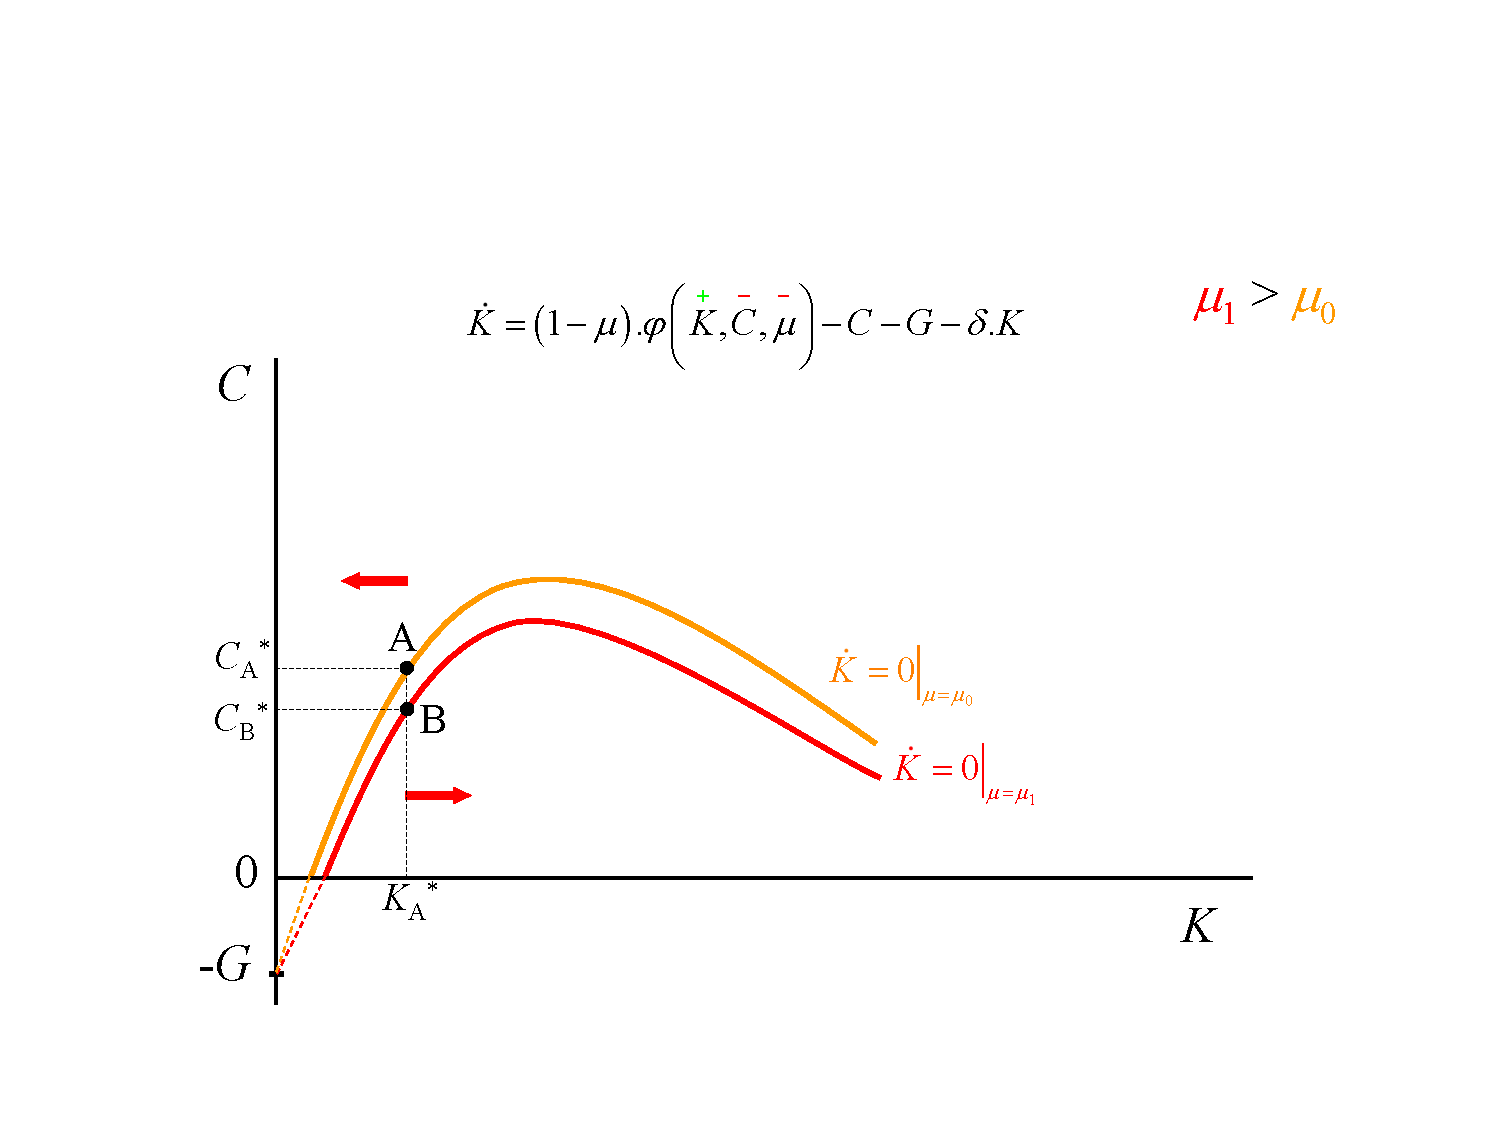
\includegraphics[max width=\linewidth]{5_0_The_New_Macroeconomics/Capital_accum_free_entry.pdf}
    \caption{Capital Accumulation with free entry}
    \label{Capital_Acc_free_entry}
\end{figure}

\paragraph{}
In order to get an equilibrium mapping capital and consumption, we'll reduce the equations of the model to take only these two variables into account, with the others still being relevant and having an impact, but getting a simpler model. 

\begin{equation*}
    r=R-\delta \implies r=(1-\mu).MPK-\delta
\end{equation*}
\begin{equation*}
    V'(1-L)=C^{-\theta}.w=C^{-\theta}(1-\mu).MPL(K,L)
\end{equation*}
\begin{equation*}
    L=\mathcal{L}(C,K,\mu)
\end{equation*}
$\mathcal{L}$ variates positively in $K$, and negatively in $C$ and $\mu$.
Replacing the L in $MPK(K,L)$ in $r$ by $\mathcal{L}$:
\begin{equation*}
        r=(1-\mu).MPK(K,\mathcal{L}(C,K,\mu))-\delta 
\end{equation*}
\begin{equation*}
        r=(1-\mu).\varphi_{K}(C,K,\mu)-\delta
\end{equation*}
Inserting these into the consumption Euler equation: 
\begin{equation*}
    \frac{\dot{C}}{C}=\frac{1}{\theta}\bigg[(1-\mu)\varphi_{K}(C,K,\mu)-\delta-\rho \bigg]
\end{equation*}
Note that $\varphi_{K}$ varies negatively on all parameters. 
\begin{figure}[H]
    \centering
    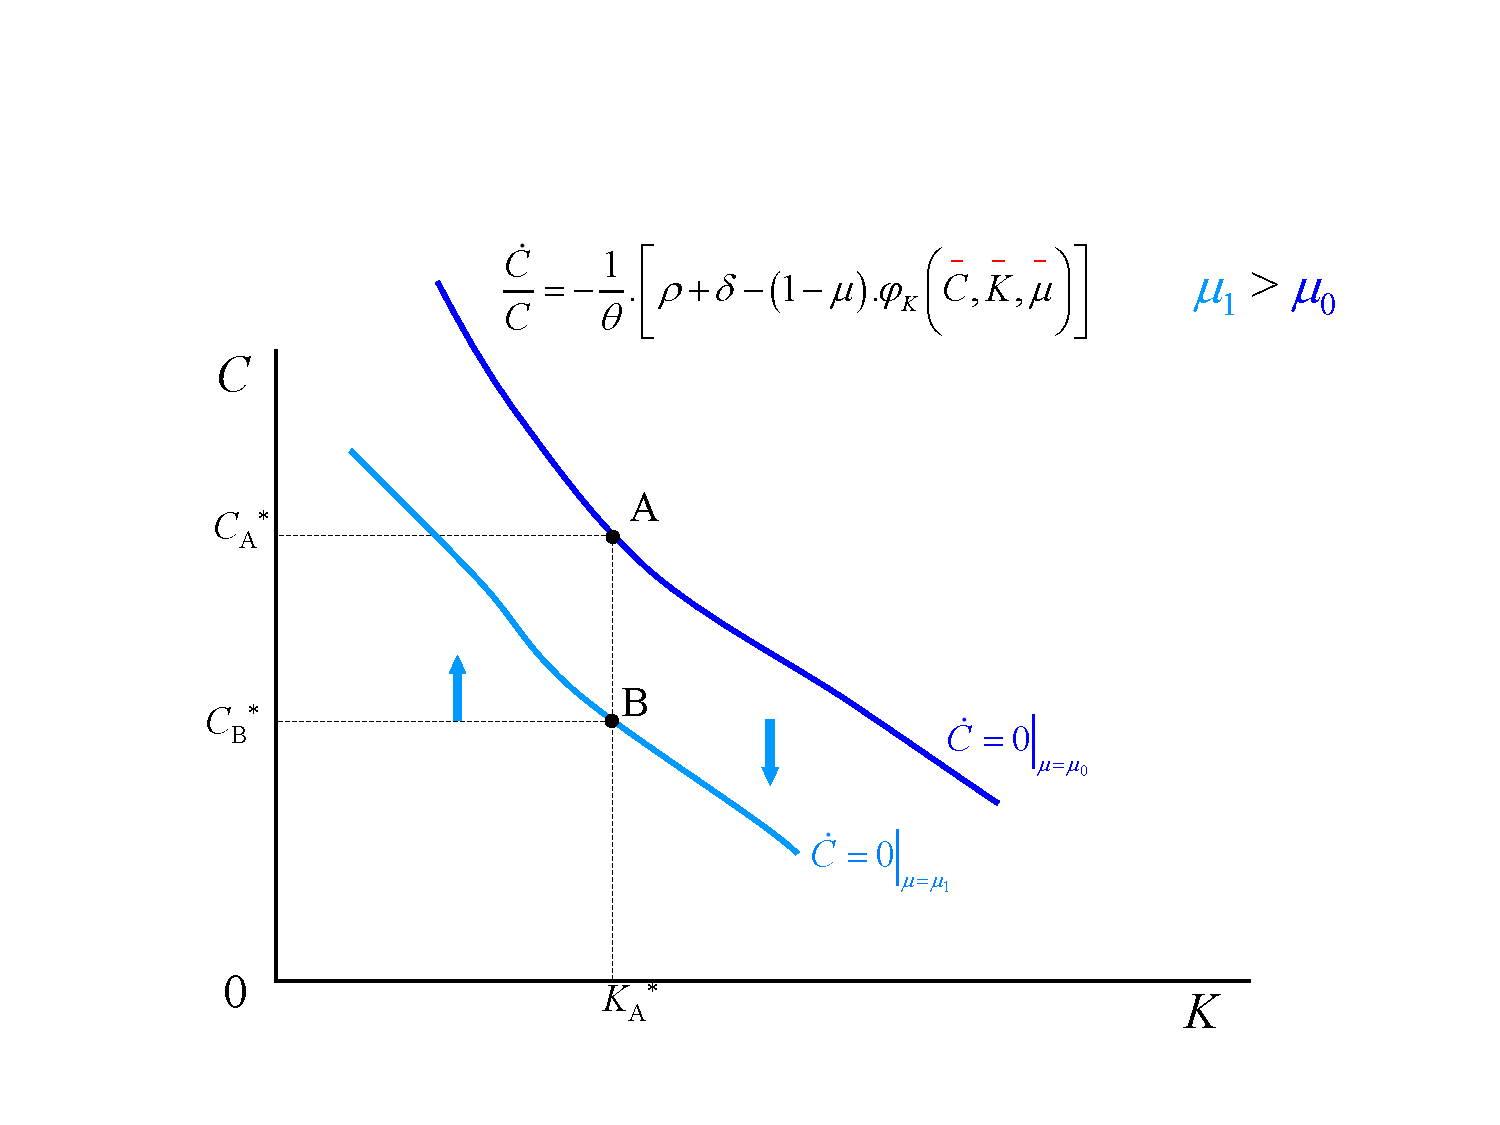
\includegraphics[max width=\linewidth]{5_0_The_New_Macroeconomics/Consumption_Euler_graph.pdf}
    \caption{Consumption Euler Equation and the Markup}
    \label{Consumption_Euler_Eq_Markup}
\end{figure}

 \paragraph{Steady State}
At a SS, $\dot{C}=0 \implies \varphi_{K}(C,K,\mu)=\frac{\rho+\delta}{1-\mu}$. 

\begin{equation*}
    F(K,L)=F(K,\mathcal{L}(C,K,\mu))=\varphi(K,C,\mu)
\end{equation*}
$\varphi(C,K,\mu)$ varies negatively in $\mu$ and $C$ because a higher $\mu$ or higher consumption result in less employment, and hence, less production. Varies positively in $K$ because more capital turns into more output. 

\begin{equation*}
\dot{C}=\dot{K}=0 \\
\implies C^{*}=\mathcal{C}(K^{*},\mu,G^{*})
\end{equation*}

$\mathcal{C}$ is positively impacted by $K^{*}$ and negatively by $\mu$ and $G^{*}$. 
In equilibrium:

\begin{equation*}
        (1-\mu)MPK(K^{*},L^{*})=\rho+\delta \\
\end{equation*}
\begin{equation*}
        (1-\mu)MPK \bigg[K^{*},\mathcal{L}(\mathcal{C}(K^{*},\mu,G^{*}),K^{*},\mu \bigg]=\rho+\delta
\end{equation*}
Define $\xi(K^{*}, \mu,G^{*})$, as $\xi(K^{*}, \mu,G^{*})= (1-\mu)MPK \bigg[K^{*},\mathcal{L}(\mathcal{C}(K^{*},\mu,G^{*}),K^{*},\mu \bigg]$. Capital and $\mu$ (the mark-up) have a negative impact in $\xi$, and government spending has a positive effect. 
\paragraph{}
See in the graph, a change in $\mu$ as $\mu_{1}>\mu_{0}$, moves $\xi$ down to the left, and makes the optimal level of capital lower.

\begin{figure}[H]
\centering
\begin{tikzpicture}[scale=1.5]

% Axis

\draw [thick](0,0) -- (8,0);

\draw [thick](0,0) -- (0,5.5);

\node [left] at (-0.2,5.3) {$\xi(K^{*},\mu,G^{*})$};

\node [below] at (8.2,-0.2) {$K$};

%Curve
\draw [thick] (1.1,5) to [out=285,in=155] (4.7,0.7) node[above]{$\xi_{1}$};
\draw [thick] (1.5,5) to [out=300,in=160] (6,1.5) node[above]{$\xi_{0}$};
\draw [thick] (0,2) -- (7,2) node[right]{$\rho+\delta$};
\draw [dashed] (2.8,2)--(2.8,0)node[below]{$K^{*}_{1}$};
\draw [dashed] (4.85,2)--(4.85,0)node[below]{$K^{*}_{0}$} ;
\end{tikzpicture}
\caption{Optimal Capital accumulation}

\end{figure}
\paragraph{Dynamics}

\begin{figure}[H]
    \centering
    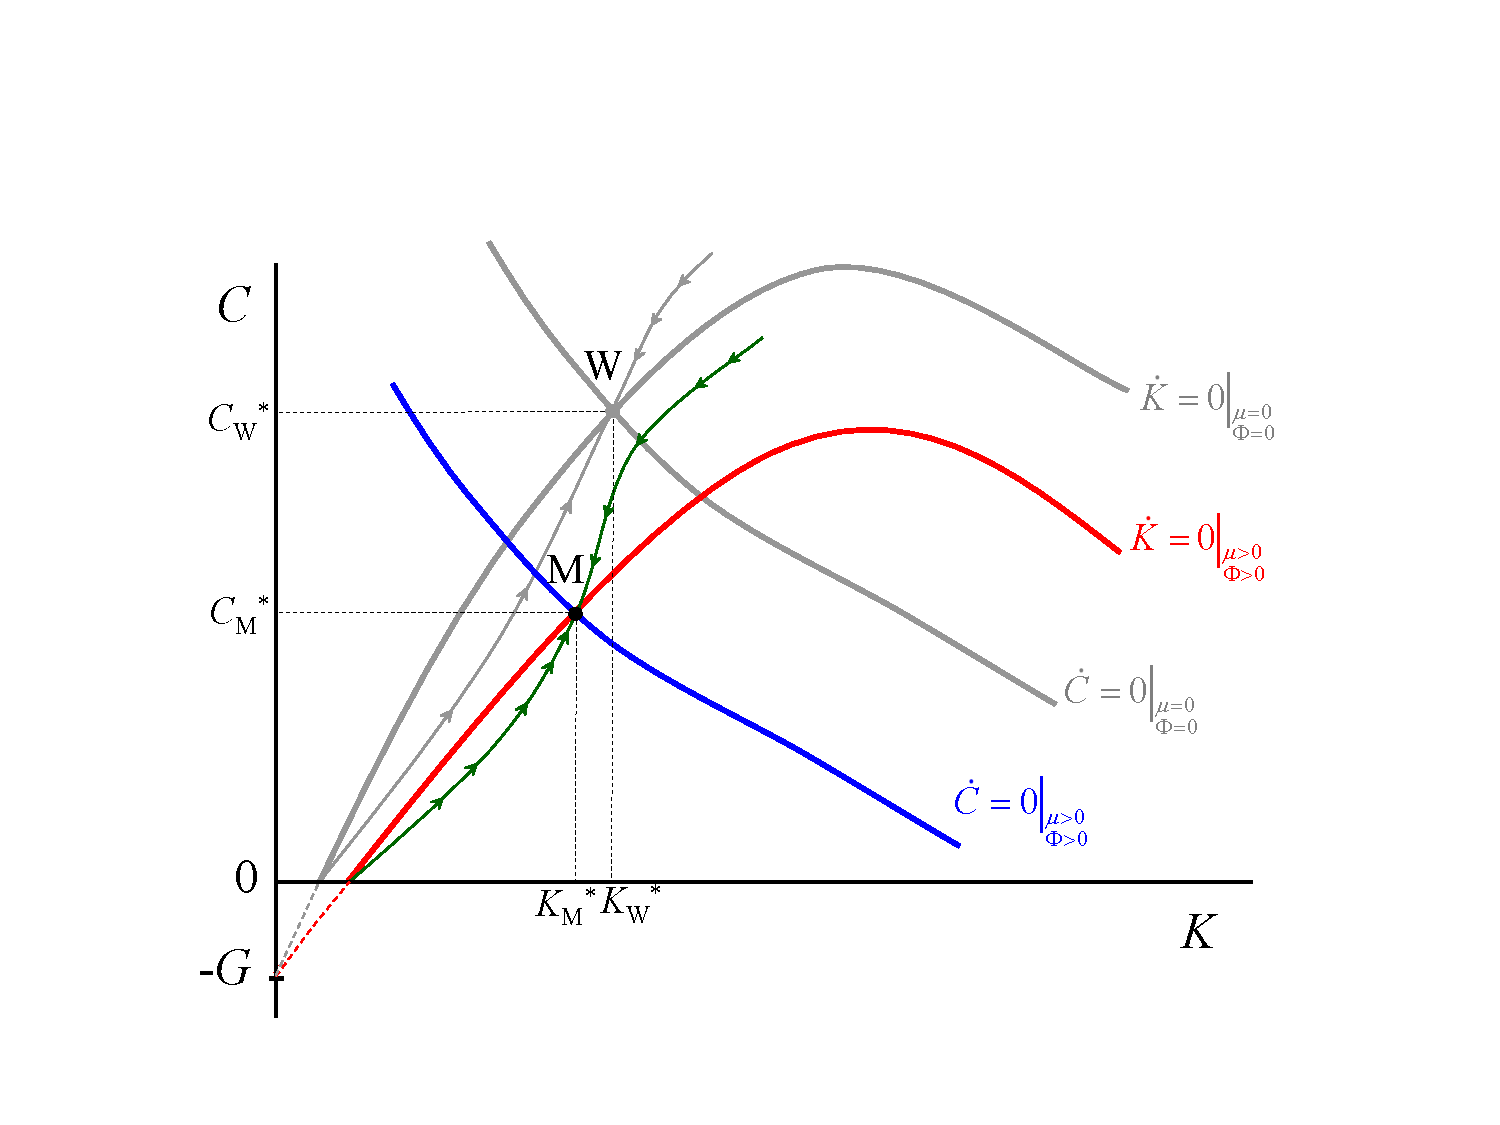
\includegraphics[max width=\linewidth]{5_0_The_New_Macroeconomics/long_run_eq.pdf}
    \caption{Long-run equilibrium in the Dixit-Stiglitz-Ramsey model with free entry}
    \label{LR_Equilibrium}
\end{figure}
Like in the Ramsay model, equilibrium isn't a single point, but an equilibrium path.

\paragraph{Fiscal Policy}

\begin{figure}[H]
    \centering
    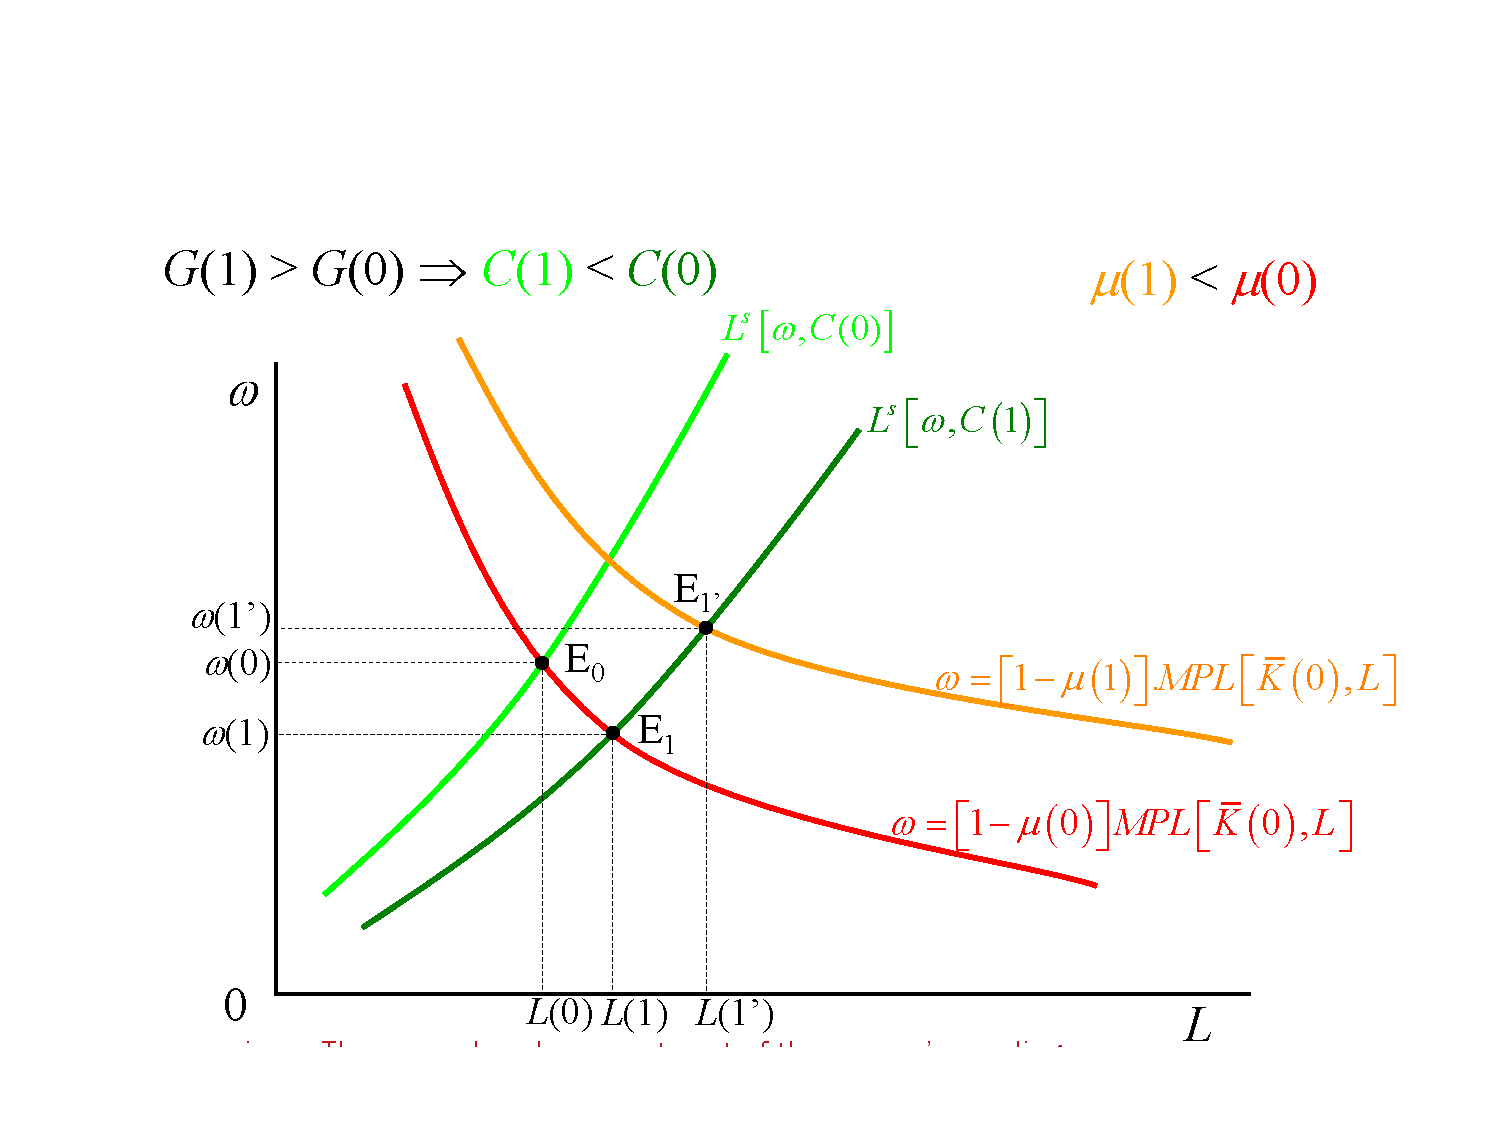
\includegraphics[max width=\linewidth]{5_0_The_New_Macroeconomics/Fiscal_Policy.pdf}
    \caption{Fiscal Policy, real wages, and the markup}
    \label{Fiscal_Policy}
\end{figure}

\paragraph{Measuring the Solow Residual} 
Introducing a measure of productivity $A$ in the production function: 
\begin{equation*}
    y(j)=A.\big[F(K(j),L(j))-\Phi \big]
\end{equation*}

And from that we get the aggregate production function: 
\begin{equation*}
    Y=A.F(K,L)-n.\Phi.A
\end{equation*}

\begin{equation*}
    \dot{Y}=\dot{A}.F+A\big[ \frac{\partial F}{\partial K}.\dot{K} + \frac{\partial F}{\partial L}.\dot{L} \big]-n.\Phi.\dot{A} 
\end{equation*}
\begin{equation*}
    \frac{\dot{Y}}{Y}=\frac{MPK.K}{Y}\frac{\dot{K}}{K}+\frac{MPL.L}{Y}.\frac{\dot{L}}{L}+\frac{(F-n\Phi).A}{Y}.\frac{\dot{A}}{A}
\end{equation*}

Note that $\frac{MPK.K}{Y}=\frac{Sh_{K}}{1-\mu}$ and $\frac{MPL.L}{Y}=\frac{Sh_{L}}{1-\mu}$.

\begin{equation*}
    g_{Y}=\frac{(1-\mu)MPK.K}{(1-\mu).Y}g_{K}+\frac{(1-\mu)MPL.L}{(1-\mu).Y}.g_{L}+g
\end{equation*}

Note that $(1-\mu)MPK=R$ and $(1-\mu)MPL=w$.

\begin{equation}\label{Output_growth}
    g_{Y}=\frac{1}{1-\mu}\big(Sh_{K}g_{K}+Sh_{L}.g_{L}\big)+g
\end{equation}

Because there can be pure profits, given the value of the markup, $Sh_{K}+Sh_{L}$ can be greater, smaller, or equal to 1, depending on the existence of pure profits. Recall $Y=w.L+R.K+\pi$; $Sh_{K}+Sh_{L}=1$ if there are no pure profits, $Sh_{K}+Sh_{L}\leq1$ if there are pure profits, and $Sh_{K}+Sh_{L}\geq 1$ if $\pi<0$.

\begin{equation*}
    \pi=y-(w.L+R.K)=\mu.A.F-n.\Phi.A
\end{equation*}
$w.L+R.K$ is the total cost (TC). This is because $\Phi$ is a total cost, but it's not necessarily a monetary cost, it's more of an inefficiency cost, resulting from the production function. This means that it's only a cost if the firm is actually producing. 

\begin{equation*}
    TC=(1-\mu).A.F
\end{equation*}
\begin{equation*}
    Sh_{L}=\frac{w.L}{Y}=\frac{w.L}{w.L+R.K}.\frac{w.L+R.K}{w.L+R.K+\pi}
\end{equation*}
The two fractions above have know values, depending on profits (for the second fraction) and on the production function you choose (for the first equation):
\[
\frac{w.L+R.K}{w.L+R.K+\pi}= \left\{
    \begin{array}{l}
         {\leq 1}  \longleftarrow \pi > 0 \\
         {= 1}   \longleftarrow \pi=0\\ 
         {\geq 1}  \longleftarrow \pi<0
    \end{array}
\right.
\]
If the production function is a Cobb-Douglas $\frac{w.L}{w.L+R.K}=1-\alpha$.

\begin{equation*}
    \frac{TC}{Y}=\frac{w.L+R.K}{Y}=\frac{(1-\mu).A.F}{A.F-n\Phi.A}=\frac{1-\mu}{1-\frac{n.\Phi.A}{A.F}} \implies A.F=Y+n.\Phi.A \implies A.F=(1-\mu)(1+\phi)
\end{equation*}
With 
\begin{equation*}
    \phi=\frac{n.\Phi.A}{Y}
\end{equation*}

For a Cobb-Douglas Production Function: 
\begin{equation*}
    Sh_{L}=(1-\alpha)(1-\mu)(1+\phi) \implies \alpha=1-\frac{Sh_{L}}{(1-\mu)(1+\phi)}
\end{equation*}

If there is free entry in the markets, in the long run profits will go to zero. In that case: 
\begin{equation*}
    \mu.A.F=n.\Phi.A \implies \mu=\frac{n.\Phi.A}{A.F} \implies \mu=\frac{\phi}{1+\phi} \implies 1-\mu=\frac{1}{1+\phi} \implies Sh_{L}=1-\alpha
\end{equation*}

Now to measure the Solow Residual (SR): 
\begin{equation*}
    SR=g_{Y}-(Sh_{L}.g_{L}+Sh_{K}.g_{K})
\end{equation*}

Replacing $g_{Y}$ by it's expression \ref{Output_growth}:
\begin{equation*}
    SR=\frac{\mu}{1-\mu}(Sh_{L}.g_{L}+Sh_{K}.g_{K})+g
\end{equation*}

\begin{equation*}
    g_{Y}=\frac{TC}{(1-\mu).Y}\bigg( \frac{w.L}{TC}.g_{L}+\frac{R.K}{TC}.g_{K}\bigg)
\end{equation*}

If the production function is a Cobb Douglas, $\frac{w.L}{TC}=1-\alpha$ and $\frac{R.K}{TC}?\alpha$. 

\begin{equation*}
    g_{Y}=(1+\phi)\big[ (1-\alpha).g_{L}+\alpha g_{K} \big]
\end{equation*}
If there is perfect competition, $\mu=0$, this is a good measure for the SR. If not, it's influenced by the business cycle, and it's no longer a good measure of the Solow Residual. 
\newline
Without free entry in the market, a marginal increase in a factor has a bigger impact on $g_{Y}$ than in perfect competition, because of increasing returns (introduced by the inclusion of $\Phi$)







